\documentclass[t]{beamer}

\mode<presentation> {
\usetheme{CambridgeUS}
}
\usepackage[utf8]{inputenc}
\usepackage[spanish]{babel}
\usepackage{amsmath}
\usepackage{graphicx} 
\usepackage{booktabs} 
\setbeamertemplate{bibliography item}{\insertbiblabel}
\numberwithin{equation}{section}
\usepackage{amsthm}




\title[Estrellas de Planck]{Estudio de Estrellas de Planck}

\author[Hernández A.]{Alejandro Hernández A. \\ {\ \\ \footnotesize Asesor: Pedro Bargueño.} } 
\institute[Uniandes]  
{\normalsize
Universidad de los Andes, Bogotá, Colombia \\ 
}
\date{Abril 7, 2015} 

\begin{document}

\begin{frame}
\titlepage 
\end{frame}

\begin{frame}
%[allowframebreaks]
\frametitle{Contenidos} 
\tableofcontents 
\end{frame}

\section{Introducción y motivación}

\begin{frame}{Introducción}
\vspace{\fill}
\begin{itemize}
\item Soluciones estáticas y esféricamente simétricas de las ecuaciones de campo de Einstein (Agujeros negros).

%Decir lo de los horizontes de eventos

\item Problemas de las singularidades en el espaciotiempo $\leftrightarrow$ Fallas de la relatividad general.

\item Agujeros negros regulares.
\end{itemize}
\end{frame}

\begin{frame}{Motivación}
\vspace{\fill}
\begin{itemize}
\item Obtener un comocimiento más profundo de la relatividad general.

\item Conocer las limitaciones y fallas de la teoría general de relatividad.

\item Entender la regularización de agujeros negros y los conceptos físicos detrás de esto.

\item Conocer un poco acerca de teoría cuántica de campos efectiva en relatividad general.

%En la medida de lo posible
\end{itemize}
\vspace{\fill}
\end{frame}


\section{\label{preliminaries section} Preliminares}


\subsection{Condiciones de energía}

%Ojo con las implicaciones
\begin{frame}{Condiciones de energía}
\vspace{\fill}
Las condiciones de energía son \cite{carroll}
\begin{itemize}
\item \textbf{NEC:} $\rho \geq 0$

\item \textbf{WEC:} $\rho \geq 0$,  $\rho + p_{i} \geq 0$ para $i \in \{1,2,3\}$.

\item \textbf{DEC:} $\rho \geq 0$,  $\rho + p_{i} \geq 0$, $\rho \geq |p_{i}|$ para $i \in \{1,2,3\}$.

\item \textbf{SEC:} $\rho + p_{i} \geq 0$ y $\rho + 3p_{i} \geq 0$.
\end{itemize}

%Relaciones DEC -> WEC -> NEC, SEC ->	NEC, SEC does not implies WEC

Para el estudio de agujeros negros regulares, la única condición de energía que nos interesa es la WEC.
\vspace{\fill}
\end{frame}

\subsection{Procedimiento General}

\begin{frame}{Procedimiento general}
Forma general del elemento de línea esféricamente siméetrico y estático:

\begin{equation}
\label{general static spherical}
ds^2 = -f(r)dt^2 + \frac{1}{f(r)}dr^2 + r^2d\Omega^2,
\end{equation}

\begin{equation}
\label{general f}
f(r) = 1 - \frac{2m(r)}{r}.
\end{equation}

En términos de $m(r)$ la WEC se expresa como \cite{vanegas-weak}

\begin{equation}
\label{mass wec ineq}
\begin{aligned}
\frac{1}{r^2}\frac{dm(r)}{dr} &\geq 0,\\
\frac{2}{r}\frac{dm(r)}{dr} &\geq \frac{d^2m(r)}{dr^2}.
\end{aligned}
\end{equation}

\end{frame}

\section{\label{previous metrics section} Métricas relevantes}


\subsection{\label{bardeen section} Métrica de Bardeen}
\begin{frame}{Métrica de Bardeen}
\vspace{\fill}
La métrica de Bardeen está dada por \cite{bardeen}
\small
\begin{equation}
\label{bardeen metric}
ds^2 = -\left( 1 - \frac{2mr^2}{(r^2 + g^2)^{3/2}} \right)dt^2 + \left( 1 - \frac{2mr^2}{(r^2 + g^2)^{3/2}} \right)^{-1}dr^2 + r^2d\Omega^2,
\end{equation}

\normalsize
\begin{equation}
f_{bardeen}(r) \underset{r \to 0}{\sim} 1 - \frac{2mr^2}{g^3} + \mathcal{O}(r^4),
\end{equation}

\begin{equation}
f_{bardeen}(r) \underset{r \to \infty}{\sim} 1 - \frac{2m}{r} + \frac{3mg^2}{r^3} + \mathcal{O}\left( \frac{1}{r^5} \right).
\end{equation}
\vspace{\fill}
\end{frame}

\begin{frame}{Métrica de Bardeen}
Para la interpretación física de la métrica de Bardeen, se requiere acoplar RG con electrodinámic no-lineal \cite{ayon-beato2000}

\begin{equation}
\mathcal{S} = \int dv \left( \frac{1}{16 \pi}R - \frac{1}{4 \pi}\mathcal{L}(F) \right),
\end{equation}

\begin{equation}
\label{nonlinear bardeen}
\mathcal{L}(F) = \frac{3}{2sg^2}\left( \frac{\sqrt{2g^2F}}{1 + \sqrt{2g^2F}} \right)^{5/2},\ s = \frac{|g|}{2m}
\end{equation}

Con el ansatzs $F_{\mu \nu} = 2 \delta^{\theta}_{\ \lbrack\mu} \delta^{\varphi}_{\ \nu\rbrack} B(r, \theta)
$,

\begin{equation*}
\frac{1}{4 \pi} \int_{S^{\infty}}\mathbf{F} = \frac{g}{4 \pi} \int_{0}^{\pi}\int_{0}^{2\pi}\sin (\theta) d\theta d\varphi = g
\end{equation*}

$ \leadsto g$ corresponde a la carga de monopolo autogravitante.
\end{frame}

\begin{frame}{Métrica de Bardeen}
Para la interpretación del carácter regular de la métrica de Bardeen

\begin{figure}[h!]
	\centering
	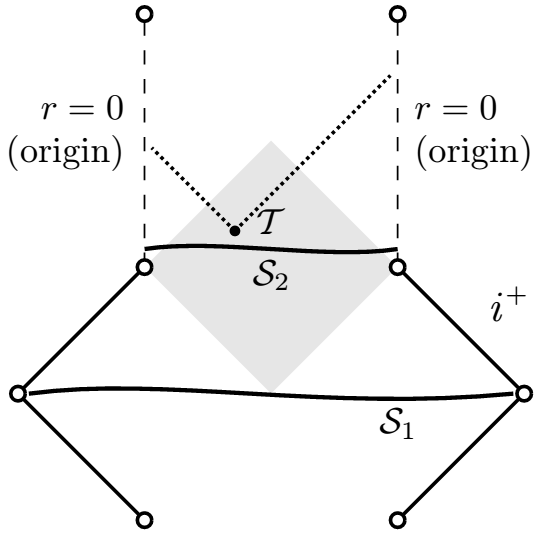
\includegraphics[width=0.35\textwidth]{bardeenDiagram}
	\caption{Estructura global de una porción del agujero negro de Bardeen. Imagen tomada de \cite{borde1994}.}
	\label{fig: bardeen diagram}
\end{figure}
\end{frame}

\begin{frame}{Métrica de Bardeen}
\vspace{\fill}
\begin{theorem}[Borde, 1996]
	\label{borde reg thm}
	Suponga que una espaciotiempo $\mathcal{M}$ satisface que
	
	\begin{enumerate}[i]
		\item contiene una superficie eventualmente futuramente atrapada $\mathcal{T}$,
		
		\item obedece la condición de convergencia nula,
		
		\item el cojunto de geodésicas nulas futuras es completo,
		
		\item su futuro causal es simple, con $E^{+}(X) \neq \emptyset,\ \forall X \subset \mathcal{M}$.
	\end{enumerate}
	
	Entonces hay una sección espacial compacta en el futuro de $\mathcal{T}$.
\end{theorem}
\vspace{\fill}
\end{frame}

\subsection{Métrica de Vaidya}

\begin{frame}{Métrica de Vaidya}
En la métrica de Schwarzschild, considerar

\begin{equation}
dt = du + \frac{dr}{(1 - 2m/r)},
\end{equation}

y al generalizar $m = m(u)$, se obtiene

\begin{equation}
\label{schw-tortoise}
ds^2 = - \left(1- \frac{2m(u)}{r}\right)du^2 - 2dudr + r^2d\Omega^2.
\end{equation}

%El SET asociado es
%
%\begin{equation}
%T_{uu} = -(m'/4 \pi r^2),\ m' = dm(u)/du
%\end{equation}
%
%corresponde a radiación saliente.

Diferencia crucial con Schwarzschild: $r = 2m(u)$ deja de ser un horizonte de eventos y se convierte en un horizonte aparente.

\begin{definition}[Horizonte aparente]
Un horizonte aparente es una hipersuperficie que separa las regiones que poseen superficies atrapadas de las regiones que no contienen este tipo de superficies.
\end{definition}

\end{frame}


\section{\label{planck stars section} Métrica de Hayward}


\subsection{Métrica de Hayward estática}

\begin{frame}{Métrica de Hayward estática}
La métrica de Hayward está dada por

\begin{equation}
\label{hayward metric}
ds^2 = -\left( 1 - \frac{mr^2}{r^3 + 2ml^2} \right) dt^2 + \left( 1 - \frac{mr^2}{r^3 + 2ml^2} \right)^{-1} dr^2 + r^2d\Omega ^2,
\end{equation}

\begin{equation}
f_{hayward}(r) \underset{r \to 0}{\sim} 1 - \frac{r^2}{l^2} + \mathcal{O}(r^5),
\end{equation}

\begin{equation}
f_{hayward}(r) \underset{r \to \infty}{\sim} 1 - \frac{2m}{r} + \frac{4l^2m^2}{r^4} + \mathcal{O}(r^{-5}),
\end{equation}

¿Interpretación física del parámetro $l$?
\
\\
\
\\
¿Cómo aplica el teorema de Borde en este caso?
\end{frame}


\subsection{Métrica de Hayward dinámica}


\section{Métrica de Hayward modificada}


\section{\label{conclusions} Conclusiones}

\section{\label{annex} Anexos}

\begin{frame}
\frametitle{Trabajo por realizar}
\vspace{\fill}
\begin{itemize}
\item Entender profundamente el teorema de Borde y sus múltiples aplicaciones en este trabajo.

\item Completar el estudio de la métrica de Hayward estática y dinámica.

%Interpretación física estilo AyónBeato y García.

\item Estudiar en detalle la métrica de Hayward modificada.

\item Interpretar físicamente la métrica de Hayward modificada.

\item Entender, en la medida de lo posible, el carácter regular de la métrica de Bardeen en términos del teorema de Borde (Anexos).

%Interpretación física del teorema

\item Entender, en la medida de lo posible, la derivación de las correcciones de teoría cuántica de campos efectiva del potencial Newtoniano (Anexos).
\end{itemize}
\vspace{\fill}
\end{frame}

\section{Referencias}
\begin{frame}{Referencias}
%[t, allowframebreaks]
\footnotesize
\bibliographystyle{unsrt}
\bibliography{Biblio}
\end{frame}
 

\begin{frame}
\Huge{
\vspace{\fill}
\centerline{
Gracias por su atención!}
}
\vspace{\fill}
\end{frame}


\end{document} 